%\documentclass{standalone}
%\usepackage{tikz}
%
%\begin{document}

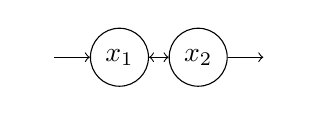
\begin{tikzpicture}
\node at (-1, 0) [shape=circle] (in) {};
\node at (-1, -0.5) [shape=circle] (out1) {};
\node at (0, 0) [shape=circle, draw] (x1) {$x_1$};
\node at (1, 0) [shape=circle, draw] (x2) {$x_2$};
\node at (2, 0) [shape=circle] (out2) {};
\draw [->] (in) to  (x1);
% \draw [->] (x1) to (out1);
\draw [<->] (x1) to (x2);
\draw [->] (x2) to (out2);
\end{tikzpicture}

%\end{document}

